% -*- Mode: LaTeX -*-

%\documentclass{sig-alternate-draft} 
%\documentclass{sig-alternate} %\newcommand{\note}[2]{}
\documentclass[11pt, draftcls, peerreview, letterpaper, onecolumn]{IEEEtran}

\newif\ifsigalt\sigaltfalse

\usepackage{supertech-sig}
\usepackage{subfigure}
\usepackage{footnote}
% \usepackage{amssymb, amsmath}

\usepackage{fullpage}
%\renewcommand{\topfraction}{0.01}% Uncomment this line to force all floats to the end if we are in submission mode
\usepackage{morefloats}% Don't complain about ``too many unprocessed floats''

%\setlength{\marginparwidth}{0.6in}
%\setstretch{1} %set to single space between lines
\setlength{\marginparwidth}{1in}
\newcommand{\note}[2]{% lines that do not end with control sequences should end with macros to avoid introducing spurious space -Bradley
    \marginpar{\color{#1}\small\raggedright#2}}%

\newcommand{\celnote}[1]{\note{blue}{CEL: #1}}
\newcommand{\yuannote}[1]{\note{green}{Yuan: #1}}
\newcommand{\racnote}[1]{\note{magenta}{RAC: #1}}


%\newcommand{\m}[1]{\mathcal{#1}}
%\newcommand{\zoid}[1]{\mathcal{#1}}
%\newcommand{\prj}[2]{\zoid{#1}_{\,#2}}
%\newcommand{\Oh}[1]{{\mathcal O}\paren{#1}}
%\newcommand{\Th}[1]{{\Theta}\left({#1}\right)}
\newcommand{\brac}[1]{\left[ #1 \right]}
\newcommand{\comb}[2]{\paren{ \begin{array}{@{}c@{}} #1 \\ #2 \end{array} }}

\def\phead#1{{\bf{#1.}}}
\newcommand{\embox}{\mbox{\hspace*{1em}}}

% \numberwithin{section}{equation}

\begin{document}

\title{The Polygonal Partial-Sum Problem}
\author{
    \IEEEauthorblockN{Yuan Tang \IEEEauthorrefmark{1} \IEEEauthorrefmark{4},
    Rezaul A. Chowdhury \IEEEauthorrefmark{2}, 
    % Steven G. Johnson \IEEEauthorrefmark{3}, \\ 
    % Bradley C. Kuszmaul \IEEEauthorrefmark{4}, 
    % Ekanathan P. Natarajan \IEEEauthorrefmark{4}} \\ 
    Charles E. Leiserson \IEEEauthorrefmark{4}} \\
    \IEEEauthorblockA{
    \IEEEauthorrefmark{1} School of Computer Science \\
        Fudan University, Shanghai 200433, P. R. China \\
        yuantang@fudan.edu.cn} \\
    \IEEEauthorblockA{
    \IEEEauthorrefmark{2} Department of Computer Science \\
        State University of New York at Stony Brook \\
        rezaul@cs.stonybrook.edu} \\
%     \IEEEauthorblockA{
%     \IEEEauthorrefmark{3} Applied Mathematics \\
%         Massachusetts Institute of Technology \\
%         stevenj@math.mit.edu} \\
    \IEEEauthorblockA{
    \IEEEauthorrefmark{4} MIT Computer Science and Artificial Intelligence Laboratory \\
        32 Vassar Street, Cambridge, MA 02139 \\
        \{yuantang, cel\}@mit.edu} \\
}

\date{}

\maketitle

% to generate a separate cover page

% \footnotenonumber{\par
%   This work was supported in part by a grant from
%   Intel Corporation and in part by the National Science Foundation
%   under Grants CCF-0937860 % HECURA
%   and CNS-1017058. % TLMM
% 
%   $\embox$Yuan Tang is Assistant Professor of Computer Science at Fudan
%   University in China and a Visiting Scientist at MIT CSAIL\@.
% %
%   Charles E. Leiserson is Professor of Computer Science and
%   Engineering at MIT CSAIL\@. }

\begin{abstract}
This paper is going to discuss about the problem derived from code clone
selection puzzle we encountered in \defn{Pochoir}'s~\cite{TangChKu11} 
development, including
the problem formulation, possible solution, and complexity bound.
\end{abstract}

\begin{IEEEkeywords}
code-clone selection puzzle, algorithm, theory, Pochoir, NP-hardness
\end{IEEEkeywords}
% LocalWords:  LocalWords Pochoir Cilk multicore

\IEEEpeerreviewmaketitle

% \category{D.1.3}{Programming Techniques}{Concurrent Programming}[Parallel programming]
% \category{D.3.2}{Programming Languages}{Language Classifications}[Specialized application languages]
% \category{G.4}{Mathematical Software}{}[Algorithm design and analysis].
% 
\secput{intro}{Introduction}

Problem formulation:

Given a $g \times m$ ($g$ rows, $m$ columns) bit-matrix, each entry of
which is either $0$ or $1$. Suppose that initially all rows and columns
are distinct, we can put ``x'' on some entries of the bit-matrix to
make these columns identical. For example, in following $3 \times 3$
bit-matrix, if we put ``x'' on entries $(2, 0)$ and $(2, 1)$ \footnote{
all coordinates of bit-matrix follows a convention in programming language
{C}}, we can make the first and second column identical like that shown
on the right-hand side.

\[ 
\begin{pmatrix} 
0 & 0 & 1 \\ 
1 & 1 & 0 \\ 
0 & 1 & 0 
\end{pmatrix}
\Longrightarrow 
\begin{pmatrix} 
0 & 0 & 1 \\ 
1 & 1 & 0 \\ 
x & x & 0 
\end{pmatrix} 
\]

However, columns such as those in pairs $(\{0, 1, x\}^T, \{0, 1, 1\}^T)$ 
or $(\{0, 1, 0\}^T, \{0, 1, x\})$ are not considered identical.

The question is: how to find the minimum number of ``x'' we should place
on any $g \times m$ bit-matrix to make the number of distinct columns
less than or equal to a given number $k$ ($k \leq m$) 
    



% introduce the concept of meta-algortihm and how to perform orthogonal
% query for d-dimensional grid, including parallelization as a sub-section
\secput{meta}{Introduction to meta-algorithm} 
% introduction to meta-algorithm, the basic notion: take one algorithm as 
% input and output another algorithm which is asymptotically better, along 
% with application in orthogonal range queries 

\subsecput{intro-meta}{Introduction to meta-algorithms and its application
to $2$-D orthogonal range queries}

In \cite{Yao82, Yao85}, A. Yao introduced an algorithm to preprocess
a $1$-D grid recursively in $O(n \alpha(n))$ space and time bound and
answer later online range queries in time $O(\alpha(n))$. A
good graphical illustration of how the algorithm works can be found
in \cite{Seidel06}. Yao's algorithm \cite{Yao82,
Seidel06} can be viewed as $1$-D meta-algorithm as defined below.
We call an algorithm a \defn{meta-algorithm} if it
takes an algorithm (called an \defn{initial algorithm}) as input, 
applies it as a black box on some
manipulated version of the input data, and effectively behaves
like a new algorithm with different (ideally improved) asymptotic 
performance bounds. The idea similar to that of a higher-order 
function in a functional language.

In this section, we demonstrate how to use the notion of meta-algorithms
to process $2$-D orthogonal range queries. Extension to higher-dimensional
grids is similar and omitted from this extended abstract due to
space limitations. In \secref{poly} we will show
how to extend it to support non-orthogonal range queries, such as triangular
and polygonal queries in $2$-D grids.

\subsubsecput{init-2D}{Initial algorithm for $2$D grids}

\punt{%
\begin{figure*}[!ht]
\centering
\includegraphics[clip,width=3in]{figures/meta_2D.eps}
\vspace{-1cm}
\caption{Meta-algorithm for $2$D orthogonal range queries}
\label{fig:meta-2D}
\end{figure*}
} %\end punt

First we need an initial algorithm to kick off. The initial algorithm 
does not need to be very efficient as long as it solve the problem
correctly. Our meta-algorithm only needs to know the complexity
bound of the initial input algorithm, but no knowledge
of any internal data structure or the internal workings
of the algorithm is needed. 
%
One such algorithm is given in \figref{init-2D-algo} of
\secref{apdx-init-2D}. 
%
The preprocessing time and space of this initial $2$-D 
algorithm $\Theta(N \log^2 N)$ for a grid of size $N$,
and the query overhead is only 3 semigroup operations. 


\punt{%
\begin{enumerate}
\item Select a longer dimension, without loss of generality, let's
  suppose it's dimension $\id{x}$.
\item Partition dimension $\id{x}$ by a center line $\overline{\id{ll'}}$
  into evenly two parts. Then all points in the grid resides
  either on the left (e.g.  $\id{p_1}$) of the center line or right
  (e.g. $\id{p_2}$). For all the points, reducing (by applying the $\oplus$
  operator) the data from center line to itself by dynamic programming.
  We call the reduced data prefix or suffix value from the center line.
\item After data reduction on both prefix and suffix values, applying Yao's
  initial $1$-D preprocessing algorithm \cite{Yao82, ChazelleRo91},
  which has complexity $O(n \log (n))$ on all lines along vertical
  dimension $\id{y}$.
\item Now we have the observation that all $2$-D orthogonal range query
  that spans across the center line $\overline{\id{ll'}}$ can be
  answered by conducting two $1$-D queries on both left-hand side
  and right-hand side of the center line. E.g. To query the rectangle
  $\Box\id{abdc}$ in \figref{init-2D}, we perform one $1$-D query
  on line $\overline{\id{l_1l_1'}}$ and another $1$-D query on line
  $\overline{\id{l_2l_2'}}$. Combining these two results by $\oplus$
  operator, we get the final query result of the orthogonal range query.
\item Recursively applying the above procedure to the left and right
  sub-grids of line $\overline{\id{ll'}}$ completes the initial algorithm
  and covers all possible range queries in the grid.
\end{enumerate}

\begin{theorem}
The preprocessing of this initial $2$-D algorithm has complexity of
$\Theta(n_1 n_2 \log (n_1) \log(n_2))$ in both time and space. 
\label{thm:init-2D-pp}
\end{theorem}

\begin{corollary}
The query overhead of this initial $2$-D algorithm is $3-\oplus$. 
\label{cor:init-2D-query}
\end{corollary}
}
% punt ends


\subsubsecput{meta-2D}{Meta-algorithm for $2$D grids}

The meta-algorithm takes one initial algorithm as input, compresses the
data alternatively along dimension $\id{x}$ or $\id{y}$ to eventually hit
the alpha bound. The description follows the notation in \figref{meta-2D}
and the pseudo-code in \figref{meta-2D-algo}.
(\figref{meta-2D} is also a graphical illustration of how the algorithm
 works) 

\begin{enumerate}
\item We start data reduction on a longer dimension,
  w.l.o.g., suppose it's dimension $\id{x}$. For
  each line of dimension $\id{y}$, partition it along dimension
  $\id{x}$ into segments of size $\id{seg\_size}$,
  which is $f_{1}(n_1)$ assuming that
  the complexity of the input algorithm ($\id{input\_2D\_algo}$) 
  is $\Theta(n_1 n_2 f_1(n_1) f_2(n_2))$.
%
\punt{
$\log (\id{x_1} - \id{x_0})$, or
  $\log^* (\id{x_1} - \id{x_0})$, $\log^{**} (\id{x_1} - \id{x_0})$,
  $\ldots$ ($\id{seg\_size}$ in \figref{meta-2D-algo}). The length of
  $\id{seg\_size}$ depends on the complexity of $\id{input\_2D\_algo}$,
  which can be a user's input parameter.
}
% punt ends
\item Apply the $\oplus$ operator to reduce
  all data within each segment into a single value. All such values
  construct a new grid --- $\id{promoted\_grid}$. Apply
  $\id{input\_2D\_algo}$ on $\id{promoted\_grid}$.
%
\item For each vertical line (along dimension $\id{y}$), reduce the
  the data relative to the left and right end of each segment (of
  size $\id{seg\_size}$) to construct $\id{prefix\_grid}$ and
  $\id{suffix\_grid}$.
%
\item For each vertical line (e.g. line $\overline{l_1l_1'}$ and
  line $\overline{l_2l_2'}$ in \figref{meta-2D}) in $\id{prefix\_grid}$
  and $\id{suffix\_grid}$, apply the $\id{input\_1D\_algo}$ on it.
  If the $\id{input\_2D\_algo}$ has bound $\Theta(n_1 n_2 f_1(n_1)
  f_2(n_2))$, the corresponding $\id{input\_1D\_algo}$ should have a bound of
  $\Theta(n f(n))$, where $f(n) \leq f_1(n)$ and $f(n) \leq f_2(n)$.
  Otherwise though the meta-algorithm will still be correct
  it won't have the desired performance bounds.
%
\item Recursively apply the meta-algorithm on segment blocks
  of size $\id{seg\_size} \times \id{n_2}$, e.g., on the colored segment block 
  $\Box \id{efgh}$ in \figref{meta-2D}.
%
\item Apply the meta-algorithm described above alternatively on dimensions
  $\id{y}$ and $\id{x}$.
%
\end{enumerate}

\begin{theorem}
Given an input $2D$ algrithm with a preprocessing complexity (in both space and time)
of $\Theta(n_1 n_2 f(n_1) f(n_2))$, where $f(n) \leq n-2$,
one round of application of the meta-algorithm
reduces the bound to $\Theta(n_1 n_2 f^*(n_1) f^*(n_2))$.
\label{thm:meta-2D-pp}
\end{theorem}

\begin{corollary}
Given an input $2D$ algrithm with a preprocessing complexity (in space and time)
of $\Theta(n_1 n_2 f(n_1) f(n_2))$, where $f(n) \leq n-2$,
and a constant query overhead,
$O(\alpha(n_1)\alpha(n_2)$ rounds of application of the meta-algorithm
reduces the preprocessing bound to $\Theta(n_1 n_2 \alpha(n_1) \alpha(n_2))$
at the cost of increasing the the query overhead to
$\Theta(\alpha(n_1)\alpha(n_2))$.
\label{cor:meta-2D-query}
\end{corollary}

More technical details, including pseudo-codes, proofs of theorems 
and corollaries, can be found in \secref{apdx-meta-intro}.
 
% introduce how to perform irregular range query by meta-algorithm
% \input{irregular} 
\secput{poly}{Polygonal Range Queries}


% introduce how to use meta-algorithm to handle irregular range queries,
% including, right triangular queries, arbitrary triangular queries, to
% arbitrary polygonal queries

In this section, we explain how use meta-algorithms
to handle polygonal range query in $2$-D grids efficiently, given all
normals are known at preprocessing time. The examples in this section are
for $2$-D, but we believe that the methodology can be extended to 
higher-dimensions (will be our future work).

\subsecput{triangle}{Triangular Query in $2$-D grid}

\begin{figure*}[t!]
\centering
\subfigure[Preparing for a 1D oblique query that returns partial-sums of trapezoidal regions]{\includegraphics[width=3in]{figures/right-triangles-1.eps}
\label{fig:init-right-triangle-1}}
\hfill
%\hspace{0.01cm}
\subfigure[Decomposing a right triangular query into oblique and rectangular queries]{\includegraphics[width=3in]{figures/right-triangles-2.eps}
\label{fig:init-right-triangle-2}}
\vspace*{-0.5cm}
%\hfill
%\subfigure[Meta-algorithm for right triangular query in $2$-D grid]{\includegraphics[width=2in]{figures/meta_right_triangle.eps}
%\label{fig:meta-right-triangle}}
\caption{Handling right triangular queries with horizontal bases and hypotenuses with a fixed slope.}
\label{fig:right-triangle}
\end{figure*}


We will first consider right triangular queries with fixed slopes.
We assume that the slope of the hypotenuse as well as that of the 
base (or perpendicular) are given during preprocessing time. 

\subsubsecput{rightTri}{Right Triangular Queries with Horizontal Bases}

In this section we show how to decompose a right triangular query with a
horizontal base and a hypotenuse with a fixed slope into three queries:
one 1D \defn{oblique query} (to be explained shortly), one 2D rectangular
query, and one 1D vertical range query.  We already know how to preprocess
the 2D grid to answer the last two queries using a constant number of
semigroup operations. We introduce the notion of oblique queries below,
and explain how to answer them in $O(1)$ semigroup operations, too.

We define oblique queries in a 2D grid $G$ w.r.t. a given straight line
and a given slope $m$.  W.l.o.g. our explanations below assume a vertical
line, say, $L_v$. We consider all lines with slope $m$ that pass thru
at least two grid points, and intersect $L_v$ at a point inside $G$.
Let $L_s$ be such a line (see \figref{init-right-triangle-1}).  If $L_s$
passes thru $k$ grid points (say, $p_0$, $p_1$, \ldots, $p_{k-1}$),
we divide $L_s$ into $k - 1$ segments, where segment $i \in [0, k - 2]$
is the section of the line starting from point $p_i$ and ending right
before point $p_{i+1}$. We will compute a semigroup sum $s_i$ (explained
below) for each segment $i$, and construct a range query data structure
based on these $s_i$ values to allow 1D partial-sum queries on them.
The $s_i$ values are computed as follows. Suppose $L_s$ intersects
$L_v$ at $o$. Consider a horizontal line $L_h$ through $o$. Now $s_i$
is computed based on the location of $p_i$ and $p_{i + 1}$ w.r.t. $L_h$
\punt{$L_v$}:
%
\begin{itemize}
%
\item[-] If $p_i$ is on the right of $L_v$, then $s_i$ is the sum of all
semigroup elements inside the trapezoid containing all grid points on or
below line $p_i p_{i+1}$, on or to the right of the vertical line through
$p_i$, to the left of the vertical line through $p_{i+1}$, and on or above
the horizontal line $L_h$. For example, in \figref{init-right-triangle-1},
$s_3$ is the sum of all grid points on or inside the trapezoid defined
by lines $p_3 p_4$, $p_3 a$, $p_4 c$ and $ac$, except the points on line
$p_4 c$.
%
\item[-] If $p_{i+1}$ is on the left of $L_v$, then $s_i$ is the sum of
all semigroup elements inside the trapezoid containing all grid points on
or to the right of $p_i p_{i+1}$, on or above the horizontal line through
$p_i$, below the horizontal line through $p_{i+1}$, and on or to the left
of $L_v$. For example, in \figref{init-right-triangle-1}, $s_1$ is the
sum of all grid points on or inside the trapezoid defined by lines $p_1
p_2$, $p_1 d$, $p_2 b$ and $bd$, but excluding the points on line $p_2 b$.
%
\item[-] If $p_{i}$ is on the left, but $p_{i+1}$ is on the right
of $L_v$, then $s_i$ is the sum of grid points on or inside the
right triangle defined by points $p_i$, $o$ and line $L_v$, and
the one defined by points $p_{i+1}$, $o$ and line $L_h$, excluding
the points on the vertical line through $p_{i + 1}$. Sum $s_2$ in
\figref{init-right-triangle-1} is an example.
%
\end{itemize}

Now suppose we are given a right triangular query $p_i p_j p$ whose
hypotenuse $p_i p_j$ lies on $L_s$, but $p_i$ and $p_j$ are on the
opposite sides of $L_v$. Then $p_i p_j p$ can be decomposed into
the following three queries (see, e.g., triangle $p_1 p_4 p$ in
\figref{init-right-triangle-2}).
%
\begin{itemize}
%
\item[-] An oblique query on $L_s$ from $p_i$ to $p_j$,
%
\item[-] A 2D query for the rectangular region $ocpd$, where $c$ is
the intersection point of $p_j p$ and $L_h$, and $d$ is the point of
intersection of lines $p_i p$ and $L_v$, and
%
\item[-] A 1D vertical range query from point $p_j$ to point $c$.
%
\end{itemize}
 
Since each of these queries has $O(1)$ complexity, query complexity of
$p_i p_j p$ is also $O(1)$.

An oblique query data structure for the entire grid $G$ can be constructed
as follows. First we vertically or horizontally partition $G$ into two
halves, and contruct a 1D oblique range query data structure for each
line $L_s$ of given slope $m$ that passes thru at least two grid points
and interesects the partition line inside the grid. We then preprocess
the two halves recursively.

In order to answer a right triangular query we first check if the
triangle is completely contained inside one of the two partitions of
$G$. If not, it intersects the partitioning line, and we can answer the
query as explained above. Otherwise, we move into the half that contains
the triangle, and recursively find a partition in which the triangle
intersects the partitioning line, and answer the query accordingly.

We will now analyze the preprocessing time and space required for
constructing the right triangular range query data structure. Our analysis
of preprocessing time will depend on the complexity of computing the
sum of the grid points inside the smallest right triangle of slope $m$
(where $m$ is the slope of the hypotenuse) that can be specified on the
given grid $G$. Observe that the two endpoints of the hypotenuse of such
a triangle will correspond to two consecutive grid points on an oblique
line $L_s$. Let $\Delta$ be the complexity of computing such a sum.

\begin{theorem}
The right triangular range query data structure for a 2D grid of size
$N$ can be constructed in $\Theta( N(\Delta + \log^{2}{N}))$ time and
$\Theta( N \log^{2}{N} )$ space assuming that the hypotenuse of each
query triangle has a fixed slope and the base is horizontal.
\label{thm:rightTri}
\end{theorem}
%
\begin{IEEEproof}(sketch)
%
We first construct a range query data structure for 2D rectangular queries
on the given grid $G$. As we discussed earlier such a data structure can
be constructed in $\Theta( N \log^2{N})$ time and space so that queries
can be answered in $O(1)$ semigroup operations.

Let us now consider the space complexity of the data structure for
oblique queries. We know that an oblique line passing through $k$ grid
points stores $k - 1$ semigroup elements.  Ignoring for the time being
the complexity of computing these elements, we can preprocess such a
line in $\Theta( k \log{k} )$ time and space so that 1D range queries on
those elements can be answered in $O(1)$ time. If we are preprocessing
a 2D grid $G'$ of size $N'$ at a particular level of recursion, then
the preprocessing time and space for all oblique lines for $G'$ in that
level of recursion is $\Theta\left( \sum_{ 0 \leq i < r }{ k_i \log{k_i} }
\right)$, where $r$ is the number of oblique lines and $k_i$ is the number
of grid points on the $i$-th oblique line. Observe that $\sum_{ 0 \leq
i < r }{ k_i } = N'$, and so the complexity above reduces to $\Theta(
N' \log{N'} )$.  Now since $G$ has $N$ points, and it is preprocessed
through $\log{N}$ levels of recursion, the preprocessing time and space
for $G$ is clearly $\Theta( N \log^2{N} )$.

The total time required for computing the semigroup elements (i.e.,
the $s_i$ values, see \figref{init-right-triangle-1}) can be derived as
follows. For each oblique line $L_s$, we first compute the sum of all
grid points inside each smallest triangle with hypotenuse on $L_s$. Since
there are fewer than $N$ such triangles across all oblique lines, the
total time for precomputing all of them is $O( N \Delta )$. Now observe
that the trapezoid below each $s_i$ (see \figref{init-right-triangle-1})
can decomposed into one smallest triangle and a rectangle.  The sum of
the grid points inside the rectangle can be computed in constant time
using the rectangular query data structure we already constructed.
Hence, each $s_i$ can thus be computed in $O(1)$ time.
%
\end{IEEEproof}

Observe that if $B$ and $P$ are the lengths of the base and the
perpendicular, respectively, of a smallest triangle, then $\Delta = O(
min(B, P) )$, as we can use our rectangular query data structure to
perform either $P$ horizontal 1D queries or $B$ vertical queries to
compute the sum inside the triangle. In the worst case, $\Delta = O(
min(B, P) ) = O( \sqrt{N} )$.

\punt{
\begin{figure*}[t!]
\centering
\subfigure[Initial algorithm for right triangular query in $2$-D grid]{\includegraphics[clip,width=3in]{figures/init_right_triangle.eps}
\label{fig:init-right-triangle}}
\hfill
%\hspace{0.01cm}
\subfigure[Meta-algorithm for right triangular query in $2$-D grid]{\includegraphics[clip,width=3in]{figures/meta_right_triangle.eps}
\label{fig:meta-right-triangle}
}
\caption{Initial and meta-algorithm for right triangular query in $2$-D grid}
\label{fig:right-triangle}
\end{figure*}
} % punt ends

\subsubsection*{Meta algorithm}
% for Right Triangular Query in $2$-D grid}
The meta-algorithm for right triangular query that rectilinear to
axes is very similar to that for rectangular query. So we just use a
triangular preprocessing/query algorithm as the $\id{input\_2D\_algo}$,
then everything remains the same as in meta-algorithm for rectangular
ranges.  \secref{meta-2D} explains more on how meta-algorithm works on 2D
rectangles. \figref{meta-2D} and \figref{meta-right-triangle} provides
a graphical illustration of how the meta-algorithm works on rectangles
and right triangles. More details are omitted from this extended abstract.

\begin{theorem}
If we input the above initial right triangular range preprocessing and
query algorithm to our meta-algorithm and self-apply $\Theta(\alpha^2(N))$,
times, it will achieve $\Theta( N(\Delta + \alpha^{2}{(N)}))$ time and
$\Theta( N \alpha^{2}{(N)} )$ space assuming that the hypotenuse of each
query triangle has a fixed slope and the base is horizontal. The query
overhead will become $\Theta(\alpha^2(N))$.
\label{thm:metaRightTri}
\end{theorem}

\begin{figure*}[t!]
\centering
\subfigure[A right triangle with an oblique base]{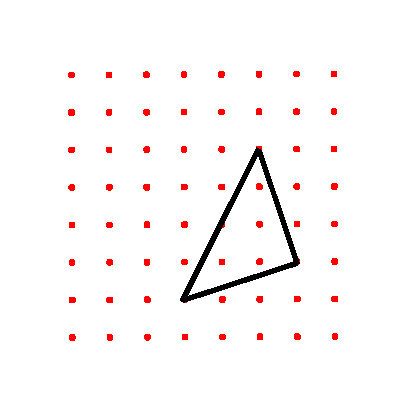
\includegraphics[width=2in]{figures/rotated-right-triangles-1.eps}
\label{fig:init-rotated-right-triangle-1}}
\hfill
%\hspace{0.01cm}
\subfigure[Rotating the input grid to make the triangle base horizontal, and embedding it in a finer grid with axis-parallel sides]{\includegraphics[width=2in]{figures/rotated-right-triangles-2.eps}
\label{fig:init-rotated-right-triangle-2}}
\hfill
\subfigure[Oblique queries in the fine grid]{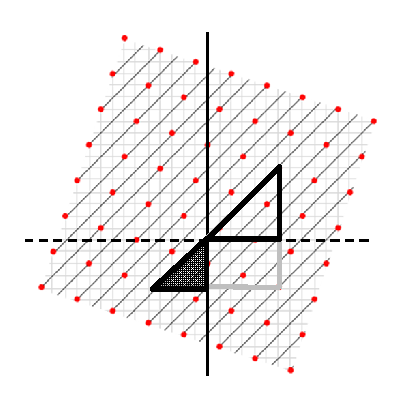
\includegraphics[width=2in]{figures/rotated-right-triangles-3.eps}
\label{fig:init-rotated-right-triangle-3}}
\caption{Handling right triangular queries with a fixed hypotenuse slope but without horizontal bases.}
\label{fig:rotated-right-triangle}
\end{figure*}


\subsubsecput{rightTriOblique}{Right Triangular Queries without Horizontal Bases}
%
In this section we consider right triangular queries that have fixed
slopes for all sides, but the base is neither horizontal nor vertical.
We define the \defn{feature size} of a straight line passing thru a
grid as the distance between two consecutive grid points lying on that
line. Let $\delta_b$, $\delta_p$ and $\delta_h$ be the feature sizes
of base, perpendicular and hypotenuse, respectively, of any query
triangle. For example, in \figref{init-rotated-right-triangle-1},
$\delta_b = \delta_p = \sqrt{10}$ and $\delta_h = \sqrt{5}$. We assume
that $\delta_b$ and $\delta_p$ are small constants.

Assuming that the original grid has $N$ points, we can rotate the grid
so that query base becomes horizontal, and embed it in an axis-parallel
finer grid of size $\Theta( N \delta_b \delta_p )$ so that every
point of the original grid sits on a grid point of the finer grid
(see \figref{init-rotated-right-triangle-2}).  Since $\delta_b$ and
$\delta_p$ are assumed to be constants, we can use our algorithm from
\secref{rightTri} to solve right triangular range queries on this grid
within the performance bounds proved in \thmref{rightTri}.

\begin{figure*}[t!]
\centering
\subfigure[An arbitrary triangle in a 2D grid]{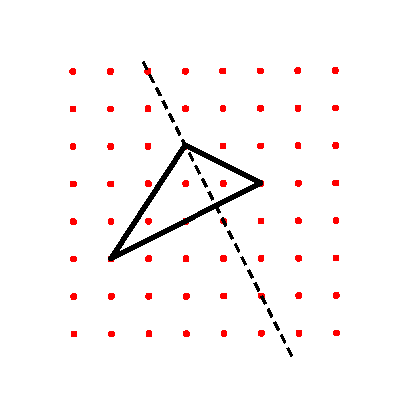
\includegraphics[width=2in]{figures/arbitrary-triangles-1.eps}
\label{fig:init-arbitrary-triangle-1}}
\hfill
%\hspace{0.01cm}
\subfigure[Rotating the grid to make the largest side of the triangle horizontal, and embedding the input grid in a finer grid with axis-parallel sides]{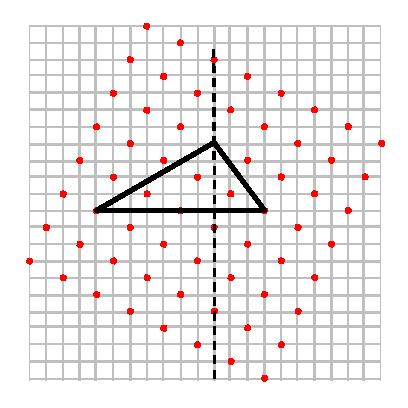
\includegraphics[width=2in]{figures/arbitrary-triangles-2.eps}
\label{fig:init-arbitrary-triangle-2}}
\hfill
%\hspace{0.01cm}
\subfigure[Decomposing an arbitrary polygonal query into rectangles and triangles using only horizontal and vertical lines]{\includegraphics[width=2in]{figures/polygonal.eps}
\label{fig:init-polygonal}}
\caption{Handling arbitrary triangular and polygonal queries with fixed slopes.}
\label{fig:rotated-arbitrary-triangle}
\end{figure*}

\subsubsecput{arbitraryTri}{Arbitrary Triangular Query in a $2$-D grid}
%
We consider arbitrary triangular queries on a 2D grid (see
\figref{init-arbitrary-triangle-1}) with fixed slopes for all sides.
We take the largest side $b$ of such a triangle, and rotate the grid so
that $b$ becomes horizontal. We embed the rotated grid in a finer grid
as in \secref{rightTriOblique} (see \figref{init-arbitrary-triangle-1}).
Let us draw a perpendicular $p$ on $b$ from the triangle vertex that
does not lie on $b$. Now assuming that the feature sizes of $b$ and
$p$ are small constants the size of the finer grid will be within a
constant factor of the size of the original grid. The perpendicular $p$
divides the query triangle into two right triangles, and thus the given
triangular query can decomposed into two right triangular queries, and
we can preprocess the finer grid to answer them within the performance
bounds proved in \thmref{rightTri}.

\subsecput{polygon}{Polygonal Query in a $2$-D grid}
%
We now consider arbitrary query polygons with sides that can have slopes
from a fixed set of slopes known during preprocessing time. We assume that
lines corresponding to these slopes have small constant feature sizes.
The key issue is decomposing this polygon into rectangles and triangles
without introducing any additional slopes. First we draw horizontal lines
through each vertex of the polygon which decompose the polygon into a set
of disjoin triangles and trapezoids (see \figref{init-polygonal}). Then we
use vertical lines to decompose each trapezoid into at most one rectangle
and no more than two right triangles. The total number of triangles and
rectangles thus created is within a constant factor of the total number
vertices in the original polygon. We now create a query data structure
for each triangle and rectangles. If the polygon has only a constant
number of vertices the performance bounds given in \thmref{rightTri} hold.

\punt{
\subsecput{extensionToHigherD}{Extension to Higher Dimensions}
%
It is not difficult to extend our 2D algorithm for right triangular
queries to trirectangular tetrahedronal queries in 3D. In a
trirectangular tetrahedron the three face angles at one vertex 
are right angles. The face opposite the vertex of the right angles 
is called the base. Similar to oblique lines parallel to
the hypotenuse of a right triangle (see \figref{right-triangle}),
we create oblique planes parallel to the base of the
trirectangular tetrahedron.  
}
% punt ends

% experimental results
\secput{expr}{Experimental Results}

% experimental results of the meta-algorithm, along with analysis

% In addition to the theoretical work, 
We have implemented our initial algorithm and meta-algorithm (pseudo-codes
in appendix \secref{apdx-init-2D} \secref{apdx-meta-2D}) for the
orthogonal range partial-sum problem on commutative semigroups.
There are empirical studies of the Range Minimum Query (RMQ)
problem \cite{FischerHe06}, which is a special case of the partial-sum
problem. But to the best of our knowledge, ours is the first experimental
study of the static partial-sum problem using an algorithm with
an $\alpha$ bound. We implemented the initial algorithm, which has
a complexity of $O(N \log^d N)$, and compared its performance with a
couple of algorithms generated by our meta-algorithm, that is, an $O(N
(\log^* N)^d)$ algorithm and an $O(N \alpha^d (N))$ algorithm.

We implemented all algorithms in {C++} standard {C++11} \cite{C++11}.
The use ``unsigned long'' as the datatype, and the partial sum operation
was simply the general integer ``+'' operation wrapped in a lambda
function and passed as a function object to all algorithms. All the query
time is calculated as an arithmetic mean of $1000$ random queries over
the entire $d$-dimensional grid.

We ran our experiments on an Intel Core i7 (Nehalem) machine.
~\footnote{Intel Xeon X5650, with clock frequency $2.66$ GHz, $32$KB L1
data cache/core, $256$KB data cache/core, $12$MB L3 cache/socket. Compiler
is icc 12.1.0.} In all performance graphs, the vertical axis is ``problem
size'' in ``unsigned long'', which is $64$-bits long, and the horizontal
axis is ``measured time'' in ``milliseconds''.  So in all performance
graphs, the closer a curve to the horizontal axis, the better the
performance of the corresponding algorithm. To verify the functional
correctness of the meta-algorithm and to compare the query overhead,
we implemented a na\"ive scan through algorithm which scans through all
the points in the query range and sums ($\oplus$) them up to answer any
online query.

From all graphs in \figref{meta-PP}, we see that the preprocessing time
of the $\alpha$ bound algorithm is always better than the $\log^*$ bound
algorithm, which, in turn, is better than the initial algorithm of $\log$
bound. So our experimental results match theoretical predictions, which
confirms the efficiency of the meta-algorithm.

From all graphs in \figref{meta-query}, we see that compared with
na\"ive scan algorithm, the query overhead of our initial algorithm or
those transformed by meta-algorithm is negligible. 
% So, it's really an $O(1)$ algorithm compared with naive scan algorithm.

In the final version, we will include more performance data
on triangular and polygonal preprocessing and query in $2$-D grids.
 
% concluding remarks
% % -*- Mode: LaTeX -*-
\secput{future}{Future Work}

Some possible future work may be:

\begin{itemize}
    \item How to relax the current constraints on polygonal range queries
    in $2$-D grids, such as arbitrary triangular queries.
    \item How to extend the polygonal range query in $2$-D to polytopal 
    range query in $3$-D grids.
\end{itemize}

\punt{In this paper, we developed a data reduction method, developed a
meta-algorithm $M$ for the partial sum query problem over $d$-dimensional
array ($d \geq 1$) of size $N$. Provided the partial sum operation is
valid over a semi-group and is associative and commutative, by taking
a user's input preprocessing algorithm $P$ of complexity $\Theta(N
\log^p N)$ in both space and time, where $0 \leq p \leq d$, and query
algorithm $Q$ of complexity $q(N, d)$, the meta-algorithm will output
a preprocessing algortihm $M(P)$ of complexity $\Theta(N \log^{p-1}
N)$,  a query algorithm $M(Q)$ with complexity $\Theta(2^{2d \cdot
\log^{*} N} \cdot q(N, d))$. Moreover, since the meta-algorithm treats
the input algorithm as a black box, if we view the meta-algorithm as a
higher-order function, by applying $M$ to $P$ at most $p$ times, i.e.
$\underbrace{M(M(\ldots M}_{p}(P)))$, we can reduce the preprocessing
complexity to optimal ($\Theta(N)$), with near-constant factor penalty on
query time (which can possibly be improved either by employing a similar
trick in \cite{AmirFiLe07} or by exploiting the internal structure of
the input query algorithm).  In addition, the result algorithm produces
good memory locality with an asymptotically smaller cache-oblivious
data structrure.}

 
% \input{ack}

\bibliographystyle{IEEEtran}
\bibliography{allpapers}

\appendix
\secput{appendix}{Appendix}

\subsecput{apdx-meta-intro}{Meta-algorithm for $2$-D grids} 

From the results in \cite{Yao82, Yao85, Seidel06}, we can establish
following recurrence for space and time bound of $1$-D
preprocessing algorithm.

\begin{eqnarray}
\mathcal{S}_{1, 0} (n) & = & n \log n \hfil \mbox{// initial algo} \\
\mathcal{S}_{1, 1} (n) & = & \Theta(n) + \mathcal{S}_{1, 0}(n/\log n) + n/\log n \cdot \mathcal{S}_{1, 1}(\log n) \hfil \mbox{// use $\mathcal{S}_{1, 0}$ inter-block query}\\
\ldots & = & \ldots \\
\mathcal{S}_{1, k} (n) & = & \Theta(n) + \mathcal{S}_{1, k-1}(n / f(n)) + n/f(n) \cdot \mathcal{S}_{1, k}(f(n)) \hfil \mbox{// Suppose the complexity of $\mathcal{S}_{1, k-1}(n) = n f(n)$} \\ 
\mathcal{S}_{1, \alpha(n)} (n) & = & \Theta(n \alpha (n)) \\ 
\label{eq:meta-1D-S1}
\end{eqnarray}

For the notation $\mathcal{S}_{d, k}$, $\mathcal{S}$ stands for the
space and time bound, the first subscript stands for dimensionality,
the second is the recursion level. Similarly, we have a recurrence
for query overhead, where $\mathcal{Q}$ stands for the query overhead,
the semantics of subscript is the same as in $\mathcal{S}_{d, k}$:

\begin{eqnarray}
\mathcal{Q}_{1, 0} & = & 1 \hfil \mbox{// initial algo}\\
\mathcal{Q}_{1, 1} & = & 2 + \mathcal{Q}_{1, 0} \hfil \mbox{// any query can be decomposed into at most one inter-block query and one suffix/prefix} \\
\ldots & = & \ldots \\
\mathcal{Q}_{1, k} & = & 2 + \mathcal{Q}_{1, k-1} \\
\mathcal{Q}_{1, \alpha(n)} & = & \Theta(\alpha(n))
\label{eq:meta-1D-Q1}
\end{eqnarray}

To extend the same kind of recurrence to multi-dimensional grids,
we start from how to use meta-algorithm to process a $2$-D
grid and iteratively apply to itself to achieve alpha bound. 
First, we need an initial algorithm to kick
off. The initial algorithm doesn't need to be very smart, it just needs
to work. Our meta-algorithm will later transform it through a series
of recursion levels and improves the asymptotic bound to eventually hit
the alpha bound.

\subsubsecput{apdx-init-2D}{Initial algorithm for $2$D grids}

\begin{figure*}[!ht]
\centering
\subfigure[Initial algorithm for $2$D orthogonal range queries]{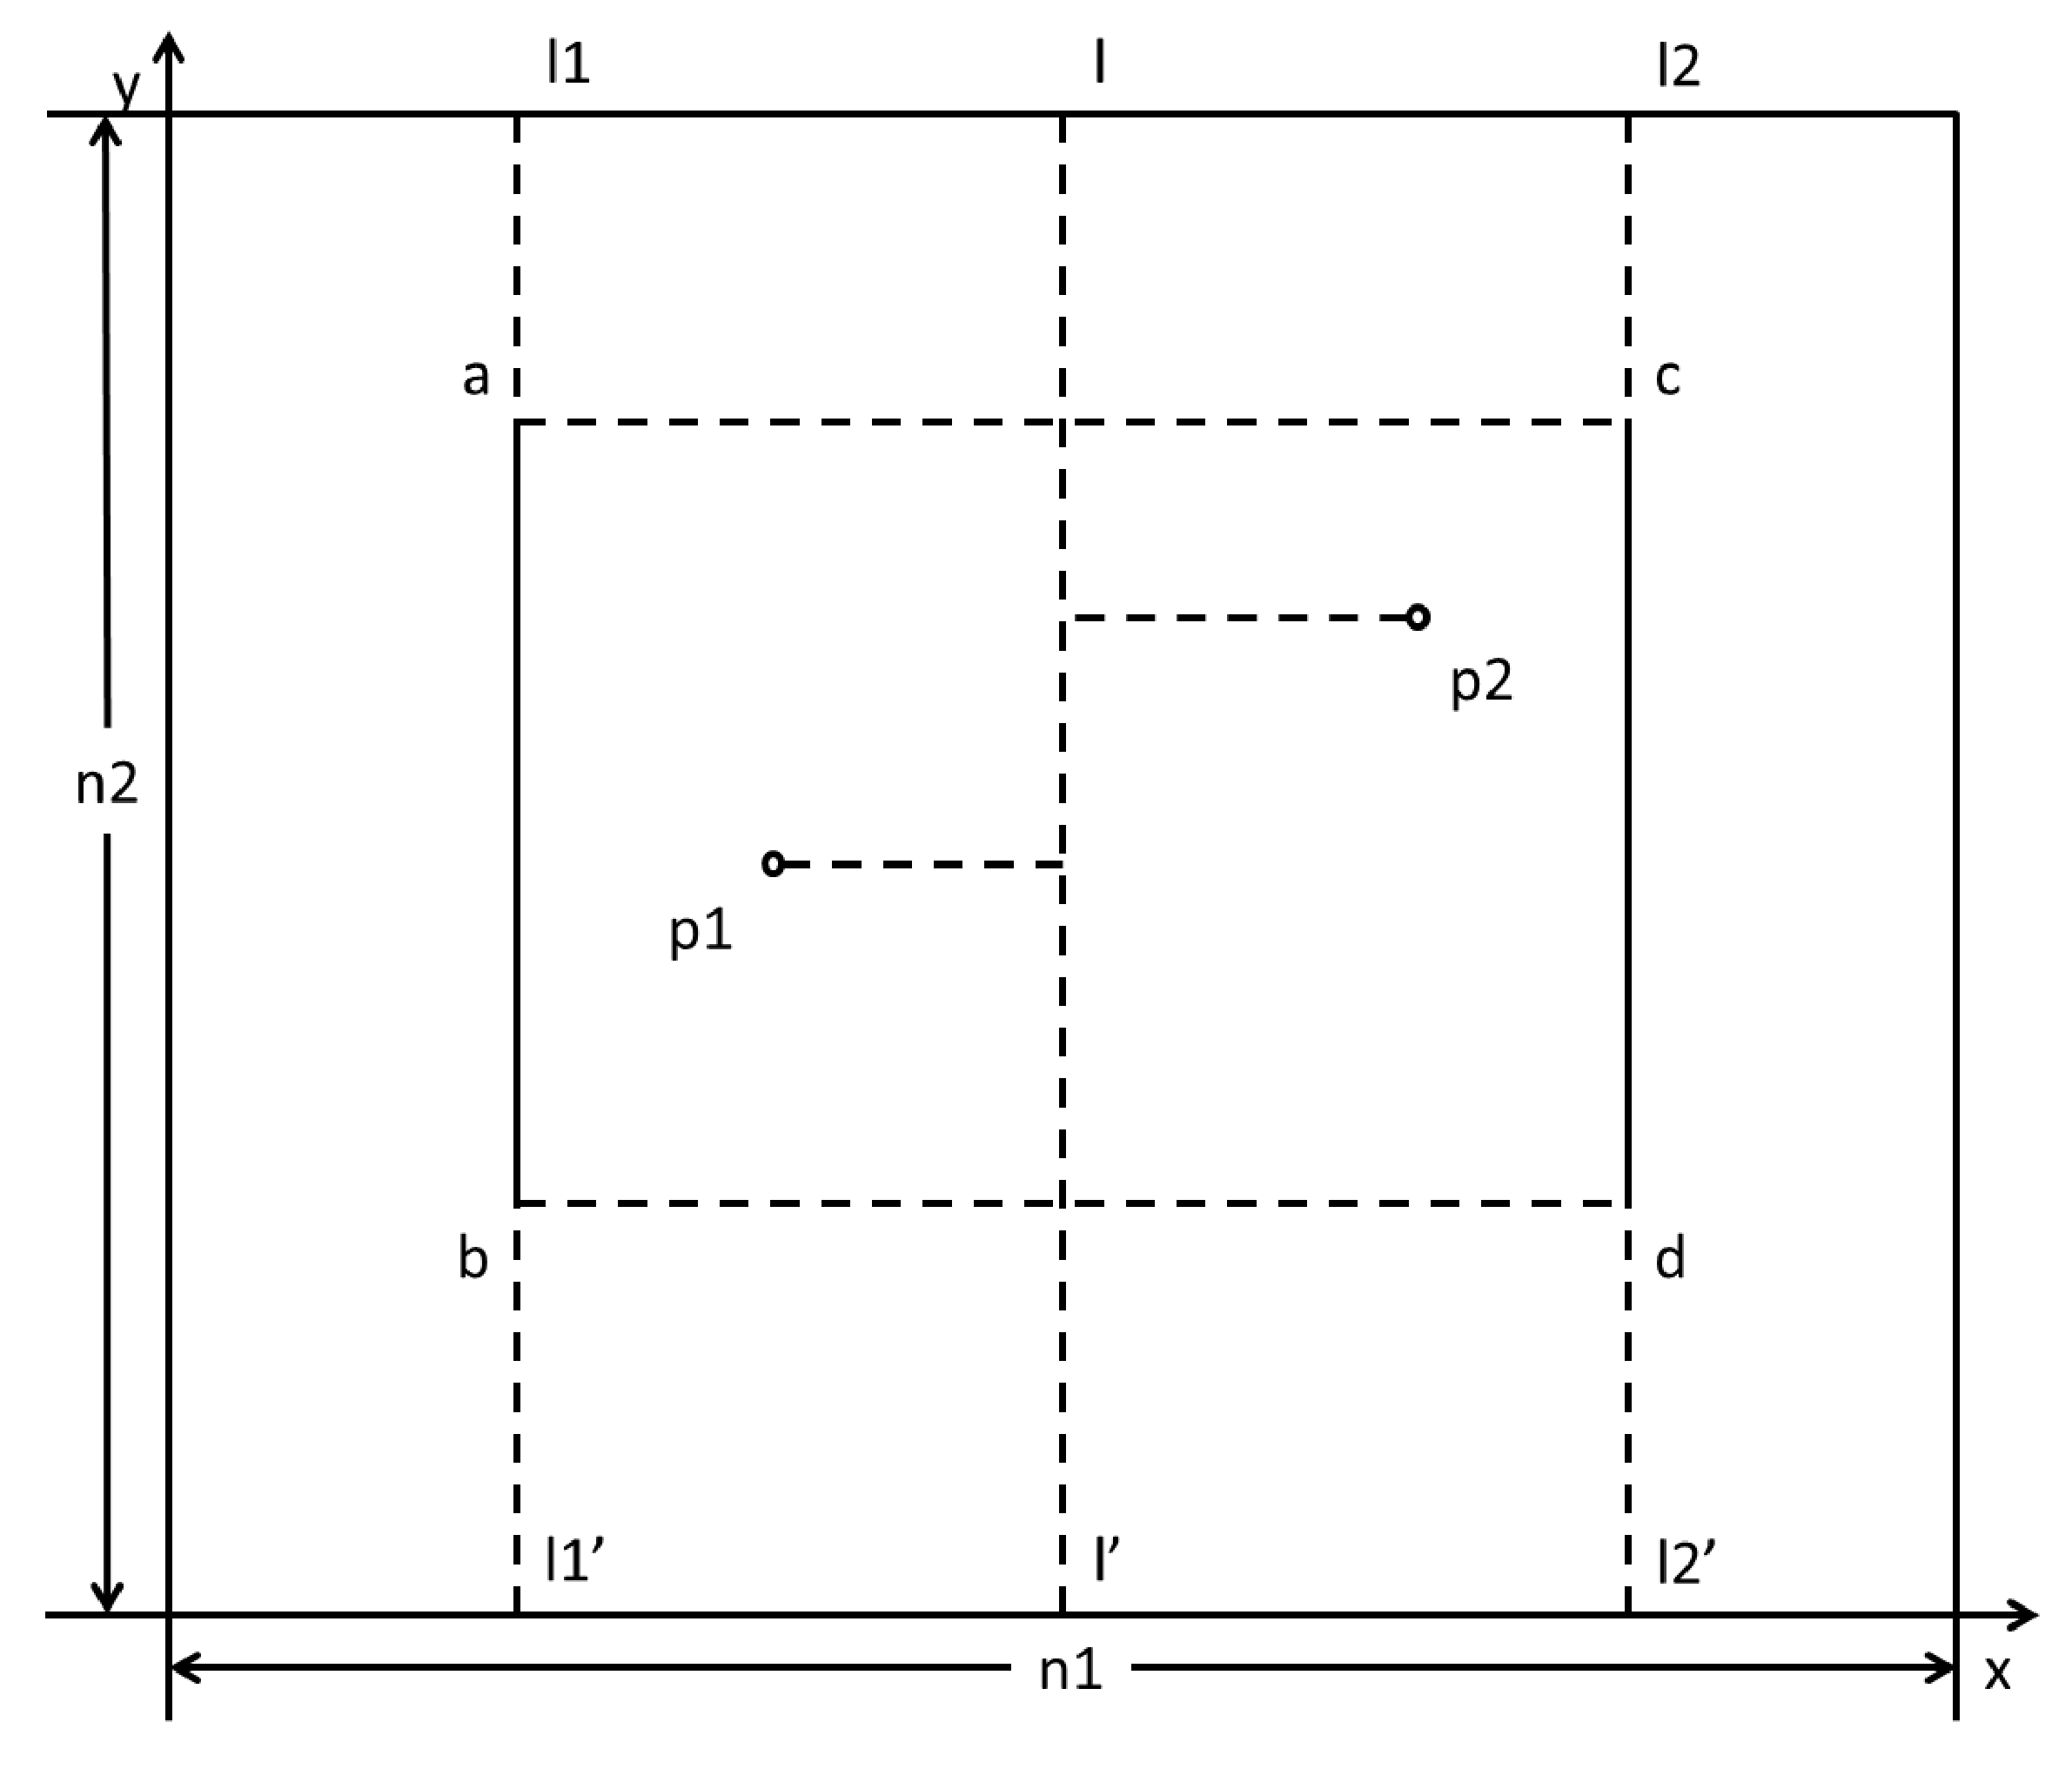
\includegraphics[clip,width=3in]{figures/init_2D.eps}
\label{fig:init-2D}}
\hfill
%\hspace{0.01cm}
\subfigure[Meta-algorithm for $2$D orthogonal range queries]{\includegraphics[clip,width=3in]{figures/meta_2D.eps}
\label{fig:meta-2D}
}
\caption{Initial and meta-algorithm for $2$-D orthogonal range queries}
\label{fig:twod}
\end{figure*}

As shown in \figref{init-2D}, the initial algorithm is a direct extension
of A. Yao's initial algorithm \cite{Yao82} to $2$-D grids. The algorithm
is diagrammed in \figref{init-2D}. The description is as follows and uses
the notation in \figref{init-2D}, the pseudo-code is in \figref{init-2D-algo}

\begin{enumerate}
\item Select a longer dimension, without loss of generality, let's
  suppose it's dimension $\id{x}$.
\item Partition dimension $\id{x}$ by a center line $\overline{\id{ll'}}$
  into evenly two parts. Then all points in the grid resides
  either on the left (e.g.  $\id{p_1}$) of the center line or right
  (e.g. $\id{p_2}$). For all the points, reducing (by applying the $\oplus$
  operator) the data from center line to itself by dynamic programming.
  We call the reduced data prefix or suffix value from the center line.
\item After data reduction on both prefix and suffix values, applying Yao's
  initial $1$-D preprocessing algorithm \cite{Yao82, ChazelleRo91},
  which has complexity $O(n \log (n))$ on all lines along vertical
  dimension $\id{y}$.
\item Now we have the observation that all $2$-D orthogonal range query
  that spans across the center line $\overline{\id{ll'}}$ can be
  answered by conducting two $1$-D queries on both left-hand side
  and right-hand side of the center line. E.g. To query the rectangle
  $\Box\id{abdc}$ in \figref{init-2D}, we perform one $1$-D query
  on line $\overline{\id{l_1l_1'}}$ and another $1$-D query on line
  $\overline{\id{l_2l_2'}}$. Combining these two results by $\oplus$
  operator, we get the final query result of the orthogonal range query.
\item Recursively applying the above procedure to the left and right
  sub-grids of line $\overline{\id{ll'}}$.
\end{enumerate}

\begin{theorem}
The preprocessing of Algoritm~\figref{init-2D} has complexity of
$\mathcal{S}_{2, 0}(n_1, n_2) = \Theta(n_1 \cdot n_2 \cdot \log (n_1)
\cdot \log(n_2))$ in both time and space.
\label{thm:init-2D-pp}
\end{theorem}

\begin{IEEEproof}
Apparently, at each level of recursion, it requires at least $n_1
n_2$ space and time to hold prefix and suffix grids.

For each vertical lines, such as $\overline{\id{l_1l_1'}}$ and
$\overline{\id{l_2l_2'}}$, we apply Yao's initial $1$-D algorithm on it, and
denote it as $\mathcal{S}_{1, 0}(n) = \Theta(n \log n)$. 

Since the partition occurs on dimension $\id{x}$, which will terminate
when the number of vertical lines in the grid less than or equal to $1$,
there are in total $\log n_1$ levels.

Combining all above calculations we have the recurrence:

\begin{eqnarray}
\mathcal{S}_{2, 0} (n_1, n_2) & = & n_1 n_2 + \log n_1 \{ n_1 \cdot \mathcal{S}_{1, 0}(n_2)\} \\
    & = & \Theta(\log n_1 n_1 n_2 \log n_2)
\label{eq:init-2D-S20}
\end{eqnarray}
\end{IEEEproof}

\begin{corollary}
The query overhead of Algorithm~\figref{init-2D} is 
$\mathcal{Q}_{2, 0} = 3-\oplus$
\label{cor:init-2D-query}
\end{corollary}

\begin{IEEEproof}
For the query, we first need to locate which recursion level the query
range resides, which is equivalent to finding the lowest common ancestor
of its range on dimension \id{x}, the overhead of which is not counted
in our simple arithmetic model.
\footnote{In RAM model, by using bit-tricks, finding lowest common
ancestor in a complete binary tree can be accomplished in $O(1)$ time} 

After locating the lowest common ancestor of the query range on dimension
\id{x}, performing two $1$-D queries on left and right-hand side of
the center line of the level, each of which requires 
$\mathcal{Q}_{1, 0} = 1-\oplus$
overhead. In the end, we need to combine both results from two $1$-D
queries into one, which requires another $1-\oplus$ operation. So in
total, we have $\mathcal{Q}_{2, 0} = 2 \mathcal{Q}_{1, 0} + 1 = 3$.
\end{IEEEproof}

\subsubsecput{apdx-meta-2D}{Meta-algorithm for $2$D grids}

The meta-algorithm takes an algorithm as input, such as the initial
algorithm described in ~\figref{init-2D} (\figref{init-2D-algo}),
compress the data alternatively on dimension $\id{x}$ or $\id{y}$ to
eventually hit the $\alpha$ bound. The description follows the notation
in \figref{meta-2D}, the pseudo-code is in \figref{meta-2D-algo}

\begin{enumerate}
\item We start data reduction on a longer dimension,
  without loss of generality, suppose it's dimension $\id{x}$. For
  each line of dimension $\id{y}$, partition it along dimension
  $\id{x}$ into segments of size $\log (\id{x_1} - \id{x_0})$, or
  $\log^* (\id{x_1} - \id{x_0})$, $\log^{**} (\id{x_1} - \id{x_0})$,
  $\ldots$ ($\id{seg\_size}$ in \figref{meta-2D-algo}). The length of
  $\id{seg\_size}$ depends on the complexity of $\id{input\_2D\_algo}$,
  which can be a user's input parameter.
\item For each segment, apply $\oplus$ operator over it and reduce
  all data within the segment into one single value. All such values
  construct a new grid --- $\id{promoted\_grid}$. Applying the
  $\id{input\_2D\_algo}$ to the $\id{promoted\_grid}$.
\item For each vertical line (along dimension $\id{y}$), reduce the
  the data relative to the left and right end of each segment (of
  size $\id{seg\_size}$ to construct the $\id{prefix\_grid}$ and
  $\id{suffix\_grid}$.
\item For each vertical line (e.g. line $\overline{l_1l_1'}$ and
  line $\overline{l_2l_2'}$ in \figref{meta-2D}) in $\id{prefix\_grid}$
  and $\id{suffix\_grid}$, apply the $\id{input\_1D\_algo}$ to it.
  If the $\id{input\_2D\_algo}$ has bound $\Theta(n_1 n_2 f_1(n_1)
  f_2(n_2))$, the corresponding $\id{input\_1D\_algo}$ should be of
  bound $\Theta(n f(n))$, where $f(n) \leq f_1(n)$ and $f(n) \leq f_2(n)$.
\item Recursively apply the meta-algorithm itself on segment blocks
  of size $\id{seg\_size} \times \id{n_2}$. E.g. on colored segment block
  $\Box \id{efgh}$ in \figref{meta-2D}
\item Repeat the above meta-algorithm alternatively on dimension
  $\id{y}$, $\id{x}$.
\end{enumerate}

\begin{theorem}
The preprocessing of Algoritm~\figref{meta-2D} has complexity of 
$\mathcal{S}_{2, \alpha(n_1) \alpha(n_2)} = \Theta(n_1
\cdot n_2 \cdot \alpha (n_1) \cdot \alpha(n_2))$ in both time and space.
\label{thm:meta-2D-pp}
\end{theorem}

\begin{IEEEproof}
\begin{enumerate}
\item In \thmref{init-2D-pp}, we proved that $\mathcal{S}_{2, 0} = 3$.
\item For recursion level $1$: we have $\mathcal{S}_{2, 0}$ as 
  $\id{input\_2D\_algo}$, and $\mathcal{S}_{1, 0}$ as $\id{input\_1D\_algo}$.
  We apply $\id{input\_2D\_algo}$ to $\id{promoted\_grid}$, which is
  of size $n_1/\log n_1 \times n_2$, and apply $\id{input\_1D\_algo}$
  to $\id{prefix\_grid}$ and $\id{suffix\_grid}$, each of which is of
  size $n_1 \times n_2$. So we have the recurrence:
    \begin{eqnarray}
      \mathcal{S}_{2, 1}(n_1, n_2) & = & \mathcal{S}_{2, 0} (n_1/\log n_1,
      n_2) + 2 \times n_1 \times \mathcal{S}_{1, 0} (n_2) 
      \frac{n_1}{\log n_1} \cdot \mathcal{S}_{2, 1}(\log n_1, n_2) \\
          & = & \Theta(n_1 n_2 \log n_2 \log^* n_1)
    \label{eq:meta-2D-S21} 
    \end{eqnarray} 
\item Solution in \eqref{meta-2D-S21} means we now have a $2$-D preprocessing
  algorithm of complexity $O(n_1 n_2 \log^* n_1 \log n_2)$ in both
  space and time. Repeat the same procedure on dimension $\id{y}$, we will 
  have the recurrence:
  \begin{eqnarray}
    \mathcal{S}_{2, 2}(n_1, n_2) & = & \mathcal{S}_{2, 1} (n_1, n_2/\log n_2) 
    + 2 \times n_2 \times \mathcal{S}_{1, 1} (n_1) 
    + \frac{n_2}{\log n_2} \cdot \mathcal{S}_{2, 2}(n_1, \log n_2) \\
        & = & \Theta(n_1 n_2 \log^* n_1 \log^* n_2) 
  \label{eq:meta-2D-S22}
  \end{eqnarray}
\item Repeat above two procedures, more generally, if we assume 
  $\id{input\_2D\_algo}$ has complexity $\Theta(n_1 n_2 f(n_1) f(n_2))$,
  where $f(n) \leq n-2$. We first segment the $2$-D grid along $\id{x}$
  dimension into size of $f(n_1)$ and supply a $1$-D algorithm of
  complexity $\Theta(n f(n))$, we will have the recurrence:
  \begin{eqnarray}
    \mathcal{S}_{2, k}(n_1, n_2) & = & \mathcal{S}_{2, k-1} (n_1/f(n_1), n_2)
    + 2 \times n_1 \times \mathcal{S}_{1, k-1} (n_2)
    + \frac{n_1}{f(n_1)} \cdot \mathcal{S}_{2, k}(f(n_1), n_2) \\
        & = & \Theta(n_1 n_2 f(n_2) f^*(n_1))
  \label{eq:meta-2D-S2k}
  \end{eqnarray}

  In a second step, we supply the $\mathcal{S}_{2, k}$ as 
  $\id{input\_2D\_algo}$ and a $1$-D algorithm of complexity 
  $\mathcal{S}_{1, k} = n f^*(n)$ as $\id{input\_1D\_algo}$.

  \begin{eqnarray}
    \mathcal{S}_{2, k+1}(n_1, n_2) & = & \mathcal{S}_{2, k} (n_1, n_2/f(n_2))
    + 2 \times n_2 \times \mathcal{S}_{1, k} (n_1) 
    + \frac{n_2}{f(n_2)} \cdot \mathcal{S}_{2, k+1}(n_1, f(n_2)) \\
        & = & \Theta(n_1 n_2 f^*(n_1) f^*(n_2))
  \label{eq:meta-2D-S2K1}
  \end{eqnarray}
\item We define the alpha function, i.e. the inverse Ackermann function to be:
  $\alpha(n) = min\{k \vert \log^{\overbrace{**\cdots*}^{k times}}(n) \leq 2\}$ 
  \cite{Seidel06}
\item Combining above steps completes the induction.
\end{enumerate}
\end{IEEEproof}

\begin{corollary}
Without loss of generality, if we assume $n_1 = n_2 = n = \sqrt(N)$, where
$N$ is the total number of points in entire grid.  The query overhead of
Algorithm~\figref{meta-2D} is $\mathcal{Q}_{2, k+1} = \Theta(\alpha^2(n))$
\label{cor:meta-2D-query}
\end{corollary}

\begin{IEEEproof}
For the query, we just need to locate which recursion level the query
range resides. At each level, the query will be decomposed into at most
three sub-queries, one $2$-D query on the $\id{promoted\_grid}$, two 
$1$-D queries on the $\id{prefix/suffix\_grid}$. If we assume that the
index calculation to locate the recursion level is free, we have following
recurrence for the query overhead:

\begin{eqnarray}
\mathcal{Q}_(2, 0) & = & 2 \times \mathcal{Q}_{1, 0} + 1 = 3 \hfil \mbox{//initial algorithm}  \\
\mathcal{Q}_(2, 1) & = & \mathcal{Q}_{2, 0} + 2 \times \mathcal{Q}_{1, 0} + 2 
    \hfil \mbox{//Decompose the query into one $2$-D query and two
    $1$-D queries} \\
\mathcal{Q}_{2, 2} & = & \mathcal{Q}_{2, 1} + 2 \times \mathcal{Q}_{1, 1} + 2 \\
\ldots & = & \ldots \\
\mathcal{Q}_{2, k}   & = & \mathcal{Q}_{2, k-1} + 2 * \mathcal{Q}_{1, k-1} + 2 \quad \mbox{//k is odd} \\
\mathcal{Q}_{2, k+1} & = & \mathcal{Q}_{2, k}   + 2 * \mathcal{Q}_{1, k} + 2 
\label{eq:meta-2D-query}
\end{eqnarray}
      
Solve the recurrence in \eqref{meta-2D-query}, we have $\mathcal{Q}_{2,
k+1} = 2 \Sigma_{i=0}^{k} \mathcal{Q}_{1, i} + 2 k$, where
$\mathcal{Q}_{1, k} = 2k + 1$ is the query overhead of $1$-D algorithm
\cite{Seidel06}.  So $\mathcal{Q}_{2, k+1} = 2 k (k+1) + 2k = \Theta(k^2)$
is the query overhead of the $2$-D meta-algorithm. Since the $1$-D
algorithm's query overhead is $\Theta(2 \alpha(n) + 1)$ \cite{Yao82,
Seidel06}, so the $2$-D meta-algorithm is $\Theta(\alpha^2(n))$
\end{IEEEproof}

\subsubsecput{apdx-init-3D}{Initial algorithm for $3$D grids}

\begin{figure}[!ht]
\centering
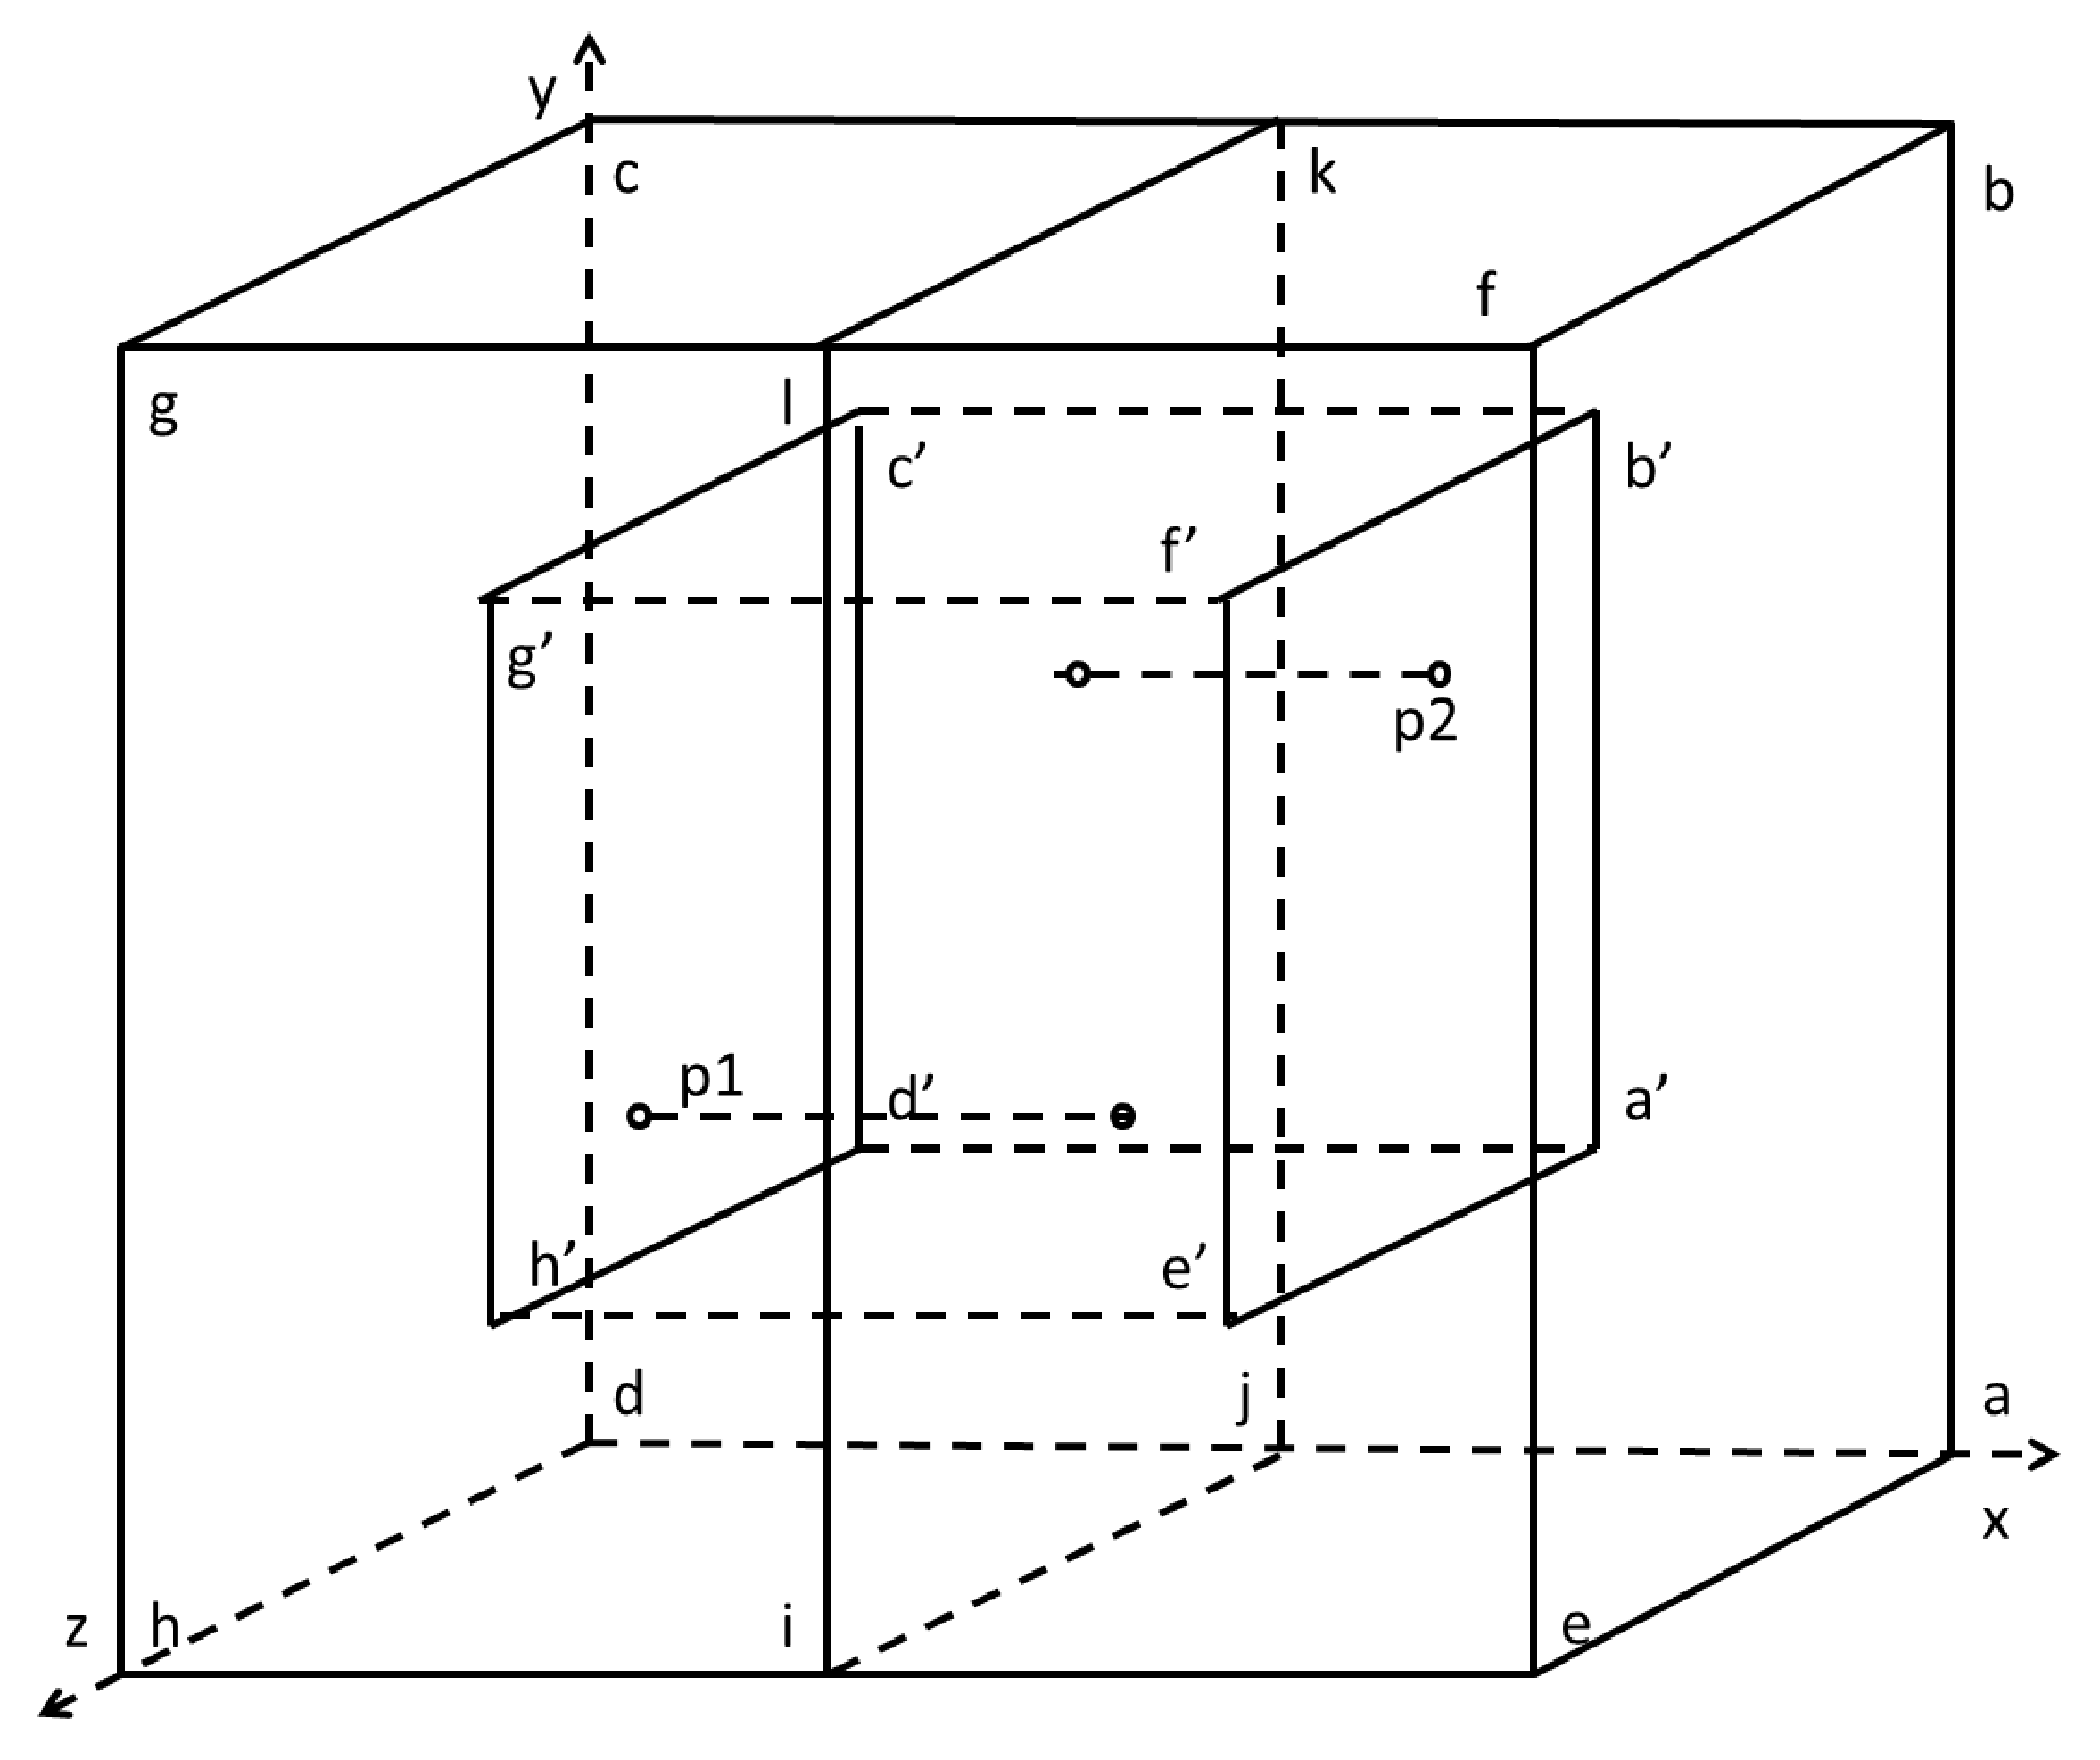
\includegraphics[width=2.5in]{figures/init_3D.eps}
\label{fig:threed}
\end{figure}

The $3$-D initial algorithm for orthogonal range query is pretty
straightforward and diagramed in \figref{threed}. Instead of center line,
we now have a center plane. In \figref{threed}, assuming $\id{x}$ is the
longest dimension and the first to reduce, we have a center face $\Box
\id{ijkl}$ to partition the entire grid into two parts. All the points
on the left-hand/right-hand side will reduce from center plane to itself
and store it as $\id{prefix/suffix\_grid}$. All the query range spanning
across the center plane can now be answered by two $2$-D queries. Then
recurse on both left and right parts of the center plane will cover all
$3$-D query ranges.

The meta-algorithm for $3$-D is also similar to the case of $2$-D, we
just need to reduce on all three dimensions to bring the preprocessing
complexity from $O(n_1 n_2 n_3 f(n_1) f(n_2) f(n_3))$ down to $O(n_1
n_2 n_3 f^*(n_1) f^*(n_2) f^*(n_3))$. The exact procedure is omitted
here.

\subsecput{init-2D}{Pseudo-code for the $2$-D initial algorithm}

\begin{figure}[!ht]
\small
\begin{codebox}
\Procname{$\proc{Init-2D}(\id{grid}, \id{x_0}, \id{x_1}, \id{y_0}, \id{y_1}; \proc{input\_1D\_algo}, \proc{op})$}
\li     $prefix\_grid \gets$ \New $((\id{x_1} - \id{x_0}) * (\id{y_1} - \id{y_0})$
\li     $suffix\_grid \gets$ \New $((\id{x_1} - \id{x_0}) * (\id{y_1} - \id{y_0})$
\li     \Comment Assuming we apply divide-and-conquer on dimension \id{x}
\li     \If $\id{x_1} - \id{x_0} <= 1$
\li         \Then \Return \Comment if the size of longer dimension $ <= 1$ then return
\li         \Else 
\li              $mid\_point \gets (\id{x_0} + \id{x_1})/2$
\li              \Comment Copy the starting point of prefix (on the right side of $mid\_point$)
\li              \Comment and suffix (on the left side of $mid\_point$)
\li              \For $y \gets \id{y_0}$ \To $\id{y_1}$
\li                  \Do $\id{suffix\_grid}[mid\_point-1][y] \gets \id{grid}[mid\_pont-1][y]$
\li                      $\id{prefix\_grid}[mid\_point][y] \gets \id{grid}[mid\_point][y]$ \End
\li              \Comment Reduce on all suffix
\li              \For $x \gets mid\_point-2$ \Downto $x_0$ 
\li                  \Do \For $y \gets \id{y_0}$ \To $\id{y_1}$
\li                      \Do $\id{suffix\_grid}[x][y] \gets \proc{op}(\id{grid}[x][y], \id{suffix\_grid}[x+1][y])$ \End \End
\li              \Comment Reduce on all prefix
\li              \For $x \gets mid\_point+1$ \To $x_1$
\li                  \Do \For $y \gets \id{y_0}$ \To $\id{y_1}$
\li                      \Do $\id{prefix\_grid}[x][y] \gets \proc{op}(\id{prefix\_grid}[x-1][y], \id{grid}[x][y])$ \End \End
\li              \Comment Apply the input $1$D algorithm on reduced prefix/suffix grid
\li              \Parfor $x \gets \id{x_0}$ \To $\id{x_1}$
\li                  \Do $\proc{input\_1D\_algo}(\id{suffix\_grid}[x][], \id{y_0}, \id{y_1}, \id{op})$
\li                      $\proc{input\_1D\_algo}(\id{prefix\_grid}[x][], \id{y_0}, \id{y_1}, \id{op})$ \End
\li              \Comment Recursively call \id{Init-2D} algorithm on the left side
\li              \Spawn $\proc{Init-2D}(\id{grid}, \id{x_0}, \id{mid\_point-1}, \id{y_0}, \id{y_1}; \id{input\_1D\_algo}, \id{op})$ 
\li              \Comment Recursively call \proc{Init-2D} algorithm on the right side
\li                     $\proc{Init-2D}(\id{grid}, \id{mid\_point}, \id{x_1}, \id{y_0}, \id{y_1}; \id{input\_1D\_algo}, \id{op})$ 
\li              \Sync \End
\end{codebox}
\caption{Initial $2$-D algorithm}
\label{fig:init-2D-algo}
\end{figure}

\subsecput{apdx-meta-2D}{Pseudo-code for the $2$-D meta algorithm}

% May put pseudo-code into appendix??
\begin{figure}[!ht]
\small
\begin{codebox}
\Procname{$\proc{Meta-2D}(\id{grid}, \id{x_0}, \id{x_1}, \id{y_0}, \id{y_1}; \id{REC}, \proc{input\_2D\_algo}, \proc{input\_1D\_algo}, \proc{op})$}
\li     \Comment Asssuming we do the data reduction on dimension $\id{x}$
\li     $seg\_size \gets \log(\id{x_1} - \id{x_0})$
\li     \Comment Depending on $\id{REC}$ level, we partition the seg\_size into $\log (\id{x_1} - \id{x_0})$, or $\log^* (\id{x_1} - \id{x_0})$, $\log^{**} (\id{x_1} - \id{x_0})$, $\ldots$
\li     \For $i \gets 0$ \To $REC$ 
\li         \Do $seg\_size \gets * seg\_size$ \End
\li     $n\_segs \gets (\id{x_1} - \id{x_0})/seg\_size$
\li     $promoted\_grid \gets $ \New $(n\_segs * (\id{y_1} - \id{y_0}))$
\li     $prefix\_grid \gets $ \New $((\id{x_1} - \id{x_0}) * (\id{y_1} - \id{y_0}))$
\li     $suffix\_grid \gets $ \New $((\id{x_1} - \id{x_0}) * (\id{y_1} - \id{y_0}))$
\li     \For $i \gets 0$ \To $n\_segs$
\li         \Do \For $j \gets 0$ \To $\id{y_1} - \id{y_0}$
\li             \Do \Comment $\proc{Reduce}$ apply input partial sum operator $\proc{op}$ over range $[i*seg_size, (i+1)*seg_size][j]$ 
\zi                 \Comment and return the reduced result into $promoted\_grid[i][j]$
\li                 $promoted\_grid[i][j] \gets \proc{Reduce}(i, j, \proc{op})$ 
\li                 \Comment $\proc{Reduce\_prefix}$ apply input partial sum operator $\proc{op}$ over range $[i*seg\_size, (i+1)*seg\_size][j]$ 
\zi                 \Comment and reduce the data relative to the beginning point of the segment ($i*seg_size$)
\li                 $prefix\_grid[i][j] \gets \proc{Reduce\_prefix}(i, j, \proc{op})$
\li                 \Comment $\proc{Reduce\_suffix}$ apply input partial sum operator $\proc{op}$ over range $[i*seg\_size, (i+1)*seg\_size][j]$ 
\zi                 \Comment and reduce the data relative to the end point of the segment ($(i+1)*seg_size$)
\li                 $suffix\_grid[i][j] \gets \proc{Reduce\_suffix}(i, j, \proc{op})$ \End \End
\li     \Comment Apply \proc{input\_2D\_algo} on the $promoted\_grid$
\li     $\proc{input\_2D\_algo}(promoted_grid, 0, n_segs, \id{y_0}, \id{y_1}; \id{REC-1}, \proc{input\_1D\_algo}, \proc{op})$
\li     \Parfor $i \gets 0$ \To $n\_segs$
\li         \Do \Comment Apply \proc{Meta-2D} itself onto the segments of $[i * seg\_size, (i+1) * seg\_size, \id{y_0}, \id{y_1}]$
\li             $\proc{Meta-2D}(\id{grid}, i * seg\_size, (i+1) * seg\_size, \id{y_0}, \id{y_1}; \id{REC}, \proc{input\_2D\_algo}, \proc{input\_1D\_algo}, \proc{op})$ \End
\li     \Parfor $i \gets \id{x_0}$ \To $\id{x_1}$
\li         \Do \Comment Apply the input $1$D algorithm on reduced prefix/suffix grid
\li             $\proc{input\_1D\_algo}(prefix\_grid[i], \id{y_0}, \id{y_1}, \proc{op})$
\li             $\proc{input\_1D\_algo}(suffix\_grid[i], \id{y_0}, \id{y_1}, \proc{op})$ \End
\end{codebox}
\caption{Meta $2$-D algorithm}
\label{fig:meta-2D-algo}
\end{figure}

\subsecput{apdx-meta-non-orthogonal}{Supplemental material for meta-algorithm for non-orthogonal range queries}

\begin{figure*}[t!]
\centering
\includegraphics[width=3in]{figures/meta_right_triangle.eps}
\vspace{-2cm}
\label{fig:meta-right-triangle}
\caption{Meta-algorithm for right triangular query in $2$-D grid.}
\end{figure*}

\subsecput{apdx-expr}{Experimental results of static partial sum problem}
\begin{figure*}[!ht]
\centering
\subfigure[Preprocessing time of meta-algorithm for $1$-D grid.]{\includegraphics[clip,width=3in]{figures/meta_1D_PP.eps}
\label{fig:meta-1D-PP}}
\hfill
%\hspace{0.01cm}
\subfigure[Preprocessing time of meta-algorithm for $2$-D grid]{\includegraphics[clip,width=3in]{figures/meta_2D_PP.eps}
\label{fig:meta-2D-PP}
}
\caption{Performance data of meta-algorithm's Preprocessing time for $1$-D and $2$-D grid}
\label{fig:meta-PP}
\end{figure*}

\begin{figure*}[!ht]
\centering
\subfigure[Query time of meta-algorithm for $1$-D grid]{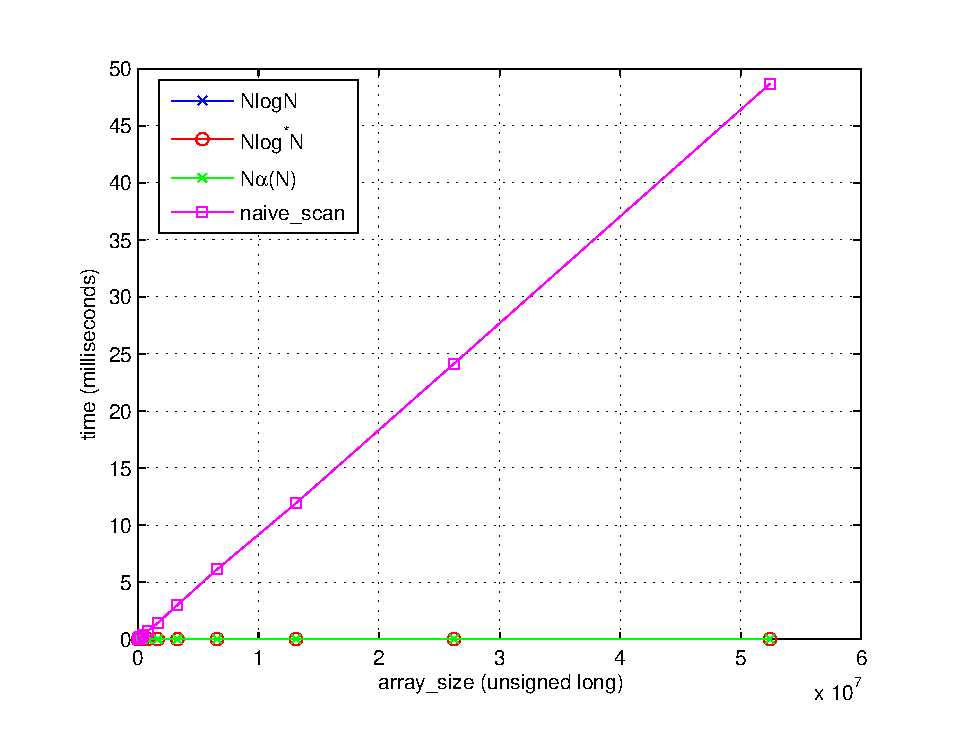
\includegraphics[clip,width=3in]{figures/meta_1D_query.eps}
\label{fig:meta-1D-query}}
\hfill
%\hspace{0.01cm}
\subfigure[Query time of meta-algorithm for $2$-D grid]{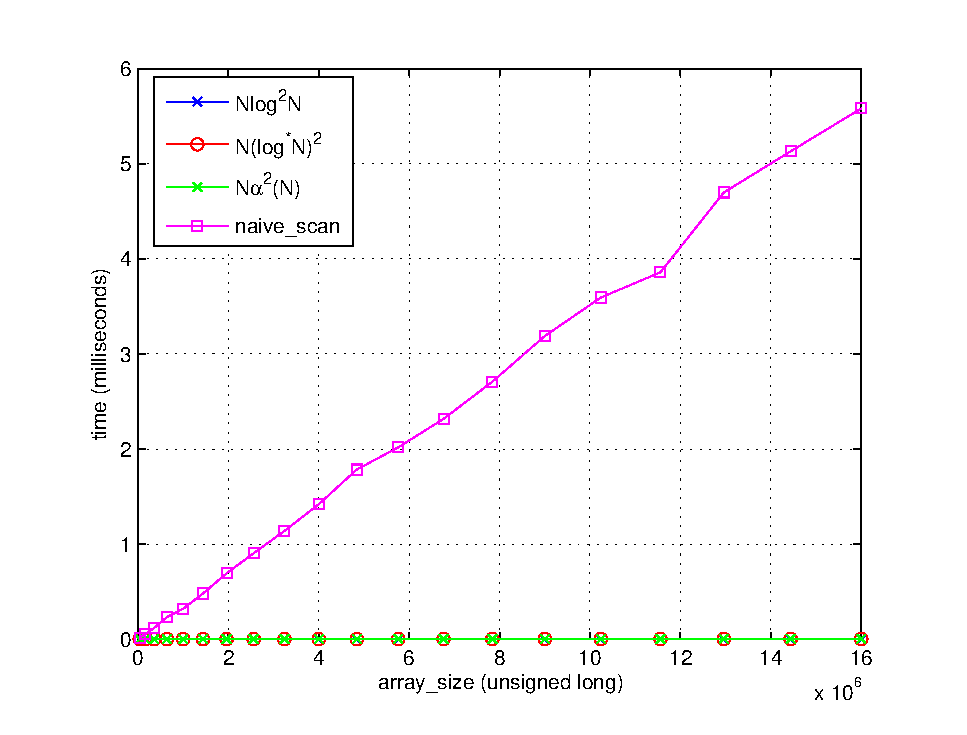
\includegraphics[clip,width=3in]{figures/meta_2D_query.eps}
\label{fig:meta-2D-query}
}
\caption{Performance data of meta-algorithm's Query time for $1$-D and $2$-D grid}
\label{fig:meta-query}
\end{figure*}




\end{document}

